\apendice{Documentación técnica de programación}

\section{Introducción}
En este anexo se describe toda la documentación técnica de programación, incluyendo la instalación del entorno de desarrollo, la estructura de archivos que hay en el repositorio de github y la integración de nuevas funcionalidades al robot.

\section{Estructura de directorios}
El repositorio del proyecto se distribuye de la siguiente manera:

\begin{itemize}
\tightlist
\item
Sprint 1: Esta carpeta contiene los códigos pertenecientes a las pruebas de funcionamiento de los componentes.
\item
Sprint 2: Esta carpeta contiene los códigos correspondientes a la prueba siguelíneas.
\item
Sprint 3: Esta carpeta contiene los códigos correspondientes a la prueba de la cuadrícula.
\item
Sprint 4: Esta carpeta contiene los códigos correspondientes con la prueba del laberinto.
\item
Sprint 5: Esta carpeta contiene el archivo main y los archivos relacionados con el desarrollo de la web.
\item
Docs: Esta carpeta contiene los archivos relacionados a la documentación como memoria y anexos.

\end{itemize}
\section{Manual del programador}

El siguiente manual tiene como objetivo servir de referencia a futuros programadores que quieran incorporar nuevas funcionalidades a PrimeBot siguiendo la estructura ya existente.
En este manual se explica como montar el entorno de desarrollo, obtener el código fuente del proyecto, compilarlo y ejecutarlo.

\subsection{Entorno de desarrollo}\label{entorno-de-desarrollo}

Para trabajar con el proyecto se necesita tener instalados los
siguientes programas y dependencias:

\begin{itemize}
\tightlist
\item
  Arduino IDE.
\item
  Visual Studio Code
\item
  Git.
\end{itemize}

A continuación se indica como instalar y configurar correctamente cada uno de ellos.

\subsubsection{Arduino IDE}\label{arduino-ide}

El principial lenguaje de programación utilizado en el proyecto de PrimeBot es Arduino (una variación de c++) y para llevar a cabo este desarrollo disponer del IDE oficial actualizado es obligatorio.

Se puede obtener para cualquier sistema directamente en la web oficial de arduino en el siguiente enlace: \href{https://www.arduino.cc/en/software}{Arduino IDE}

\begin{figure}[h]
	\centering
	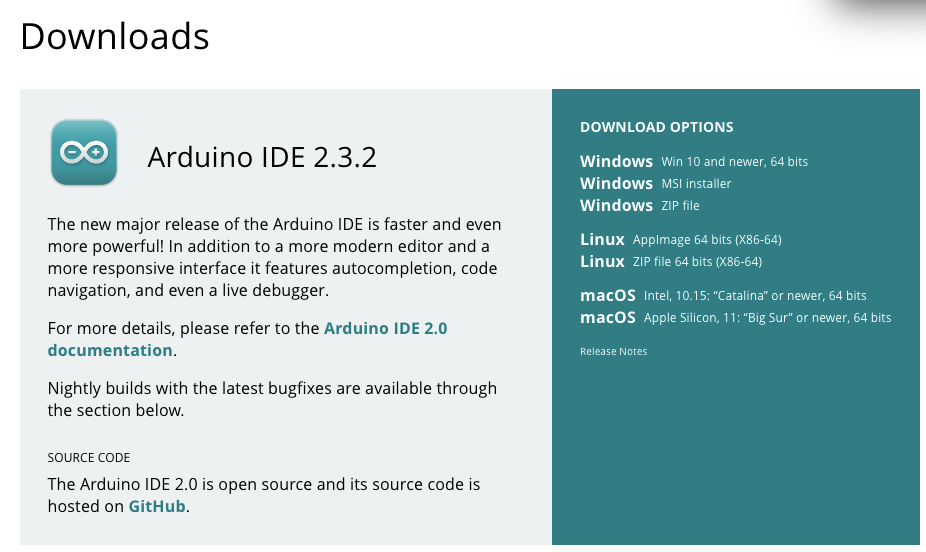
\includegraphics[width=0.5\textwidth]{anexos/instalacionArduino}
	\caption{Instalación de Arduino IDE}
	\label{fig:D.1}
\end{figure}

\subsubsection{Visual Studio Code}\label{visual-studio-code}

Visual Studio Code es el IDE empleado para el desarrollo y la implementación de la página web de PrimeBot.

Se puede obtener desde el siguiente enlace: \href{https://code.visualstudio.com/download}{Visual Studio Code}

\begin{figure}[h]
	\centering
	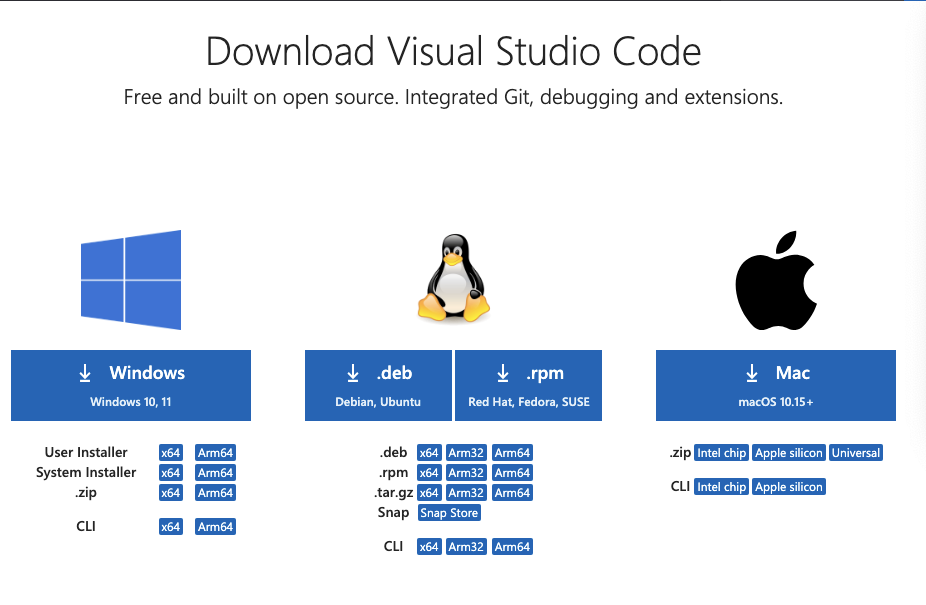
\includegraphics[width=1\textwidth]{anexos/instalacionVSCode}
	\caption{Instalación de Visual Studio Code}
	\label{fig:D.2}
\end{figure}

\subsubsection{git}\label{git}

Para hacer uso del repositorio se necesita tener instalado el gestor de versiones Git. Este programa permite clonar el repositorio, movernos dentro de el... etc.

Se puede obtener desde: \href{https://www.git-scm.com/downloads}{GIT}

Cuando esté instalado, trabajaremos con Git Bash.

\begin{figure}[h]
	\centering
	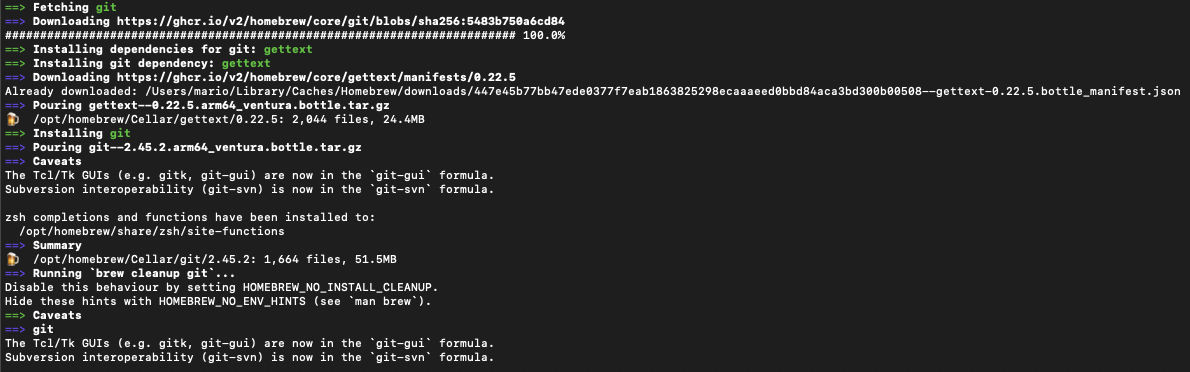
\includegraphics[width=1\textwidth]{anexos/instalacionGit}
	\caption{Instalación de Git}
	\label{fig:D.3}
\end{figure}

\subsection{Obtención del código fuente}\label{obtencion-del-codigo-fuente}

Para el desarrollo de los algoritmos empleados en PrimeBot se ha utilizado el repositorio Git hospedado en GitHub, lo primero es obtener una copia de la siguiente manera:
\begin{enumerate}
\def\labelenumi{\arabic{enumi}.}
\tightlist

\item
  Abrir la terminal Git Bash.
\item
  Desplazarse al directorio donde se desee copiar el repositorio
  (utilizando el comando \texttt{cd}).
  
  \item
  Introducir el siguiente comando:\\
  \texttt{git\ clone\ https://github.com/marioAlonso2122/Primebot.git}
  \item
  Se iniciará la descarga del repositorio, cuando finalice se dispondrá
  de una copia completa de este.
\end{enumerate}

\begin{figure}[h]
	\centering
	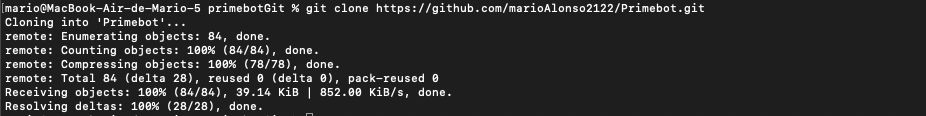
\includegraphics[width=1\textwidth]{anexos/obtenerRepositorio}
	\caption{Obtener repositorio}
	\label{fig:D.4}
\end{figure}

\subsubsection{Añadir nuevas funcionalidades}\label{nuevas-funcionalidades}

Una vez dispongamos de una copia del repositorio de PrimeBot en nuestro equipo ya podremos realizar la incorporación de nuevas funcionalidades al código de la siguiente manera:

\begin{enumerate}
\def\labelenumi{\arabic{enumi}.}
\tightlist

\item
Abrir el archivo main.ino con el editor de código Arduino.
\item
Debemos dejar las definiciones iniciales intactas ya que son los pines de las conexiones de la PCB que deben estar estáticas o PrimeBot podría dejar de funcionar.
\item
Tenemos que localizar la función llamada primeBotAction.
\item
Dentro de esta función disponemos de un recurso switch-case donde podremos incorporar nuevas funcionalidades.
\item
En el main.ino que se descargar del repositorio encontramos los 4 primeros case ya ocupados, cada valor de case corresponde a uno de los valores obtenidos a través del switch dip integrado en el PCB.
\item
Dentro del case podemos añadir nuevos valores donde incorporar nuevas funcionalidades a PrimeBot.
Se recomienda dejar un valor de case para cada funcionalidad nueva.
\item
Hay que incorporar dentro de la nueva funcionalidad un bucle while(true) que solo salga cuando se pulse el botón para poder ejecutar constantemente la funcionalidad hasta que se pulse de nuevo el botón de cambio de función.
\end{enumerate}

\begin{figure}[h]
	\centering
	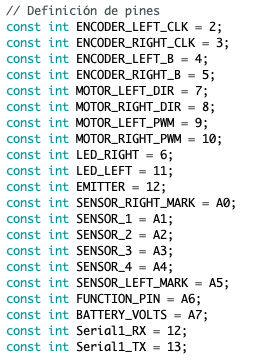
\includegraphics[width=0.5\textwidth]{anexos/definicionPines}
	\caption{Definicion de los pines de la placa en el Main}
	\label{fig:D.5}
\end{figure}

\begin{figure}[H]
	\centering
	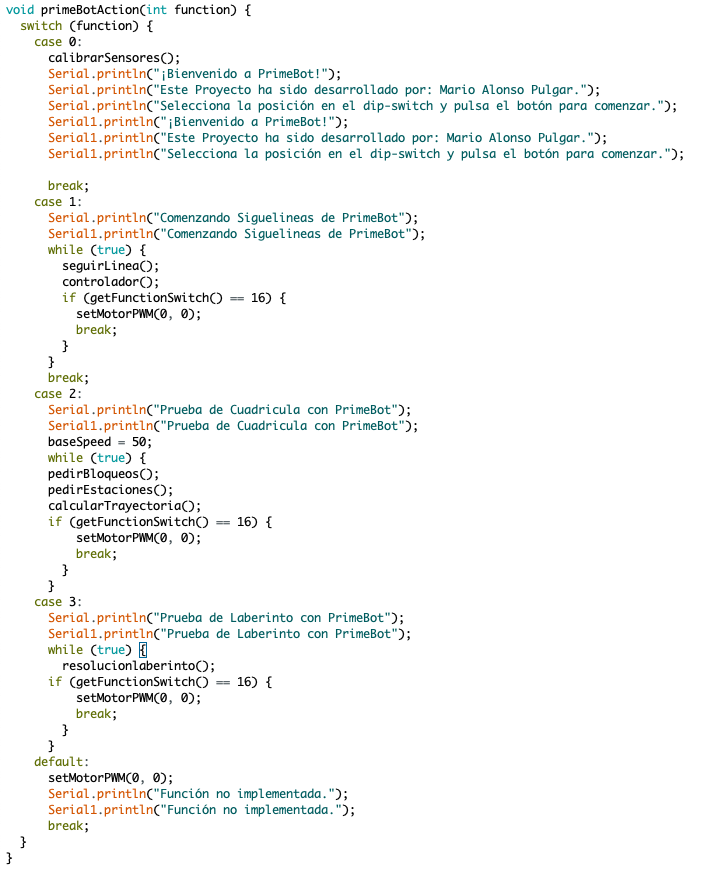
\includegraphics[width=1\textwidth]{anexos/nuevasFunciones}
	\caption{Lugar donde añadir nuevas funcionalidades}
	\label{fig:D.6}
\end{figure}


\subsubsection{Ejecutar código}\label{ejecutar-codigo}
Al estar trabajando con Arduino, el código se recomienda ejecutarlo siempre en un dispositivo real, para ello:
\begin{enumerate}
\def\labelenumi{\arabic{enumi}.}
\tightlist
\item
Conectamos la placa Arduino al equipo vía USB
\item
Dentro de las opciones del IDE de arduino en el apartado Herramientas, debemos seleccionar la placa donde vamos a cargar el código y el puerto al que está conectada esa placa.
\item
Pulsaremos en la opción subir para compilar y enviar el código a la placa arduino que vayamos a emplear.
\end{enumerate}
\begin{figure}[h]
	\centering
	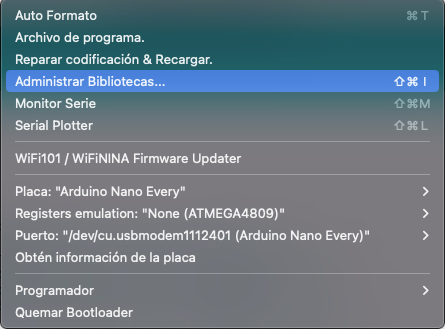
\includegraphics[width=0.5\textwidth]{anexos/seleccionarPlaca}
	\caption{Seleccion de placa en Arduino IDE}
	\label{fig:D.7}
\end{figure}
